\documentclass[letter, 12pt]{article}
% Default preamble to be included by: % Default preamble to be included by: % Default preamble to be included by: \input{preamble}

%%% Document dimensions
\usepackage[top=1in, bottom=1in, left=1in, right=1in]{geometry}
%%%

%%% Language support
\usepackage[english]{babel} % Get everything translated properly
\usepackage[latin1]{inputenc} % Input text correctly
\usepackage[T1]{fontenc} % Get hyphenation right
%%%

%%% AMS support
\usepackage{amsmath}
\usepackage{amsfonts}   % fonts
\usepackage{amssymb}    % extra symbols
\usepackage{amsthm} % Theorems
\newtheorem{theorem}{Theorem}[section]
\newtheorem{lemma}[theorem]{Lemma}
\newtheorem{proposition}[theorem]{Proposition}
\newtheorem{corollary}[theorem]{Corollary}
%%%

%%% Numbering equations
%\numberwithin{equation}{section}
%\numberwithin{equation}{subsection}
%%%

%%% tocloft
%\usepackage{tocloft}
%\renewcommand{\cftpartleader}{\cftdotfill{\cftdotsep}} % for parts
%\renewcommand{\cftchapleader}{\cftdotfill{\cftdotsep}} % for chapters
%\renewcommand{\cftsecleader}{\cftdotfill{\cftdotsep}} % for sections
%%%

%%% Typeset source code listings
\usepackage{listings}
%%%

%%% Customising captions in floating environments.
\usepackage{caption}
%%%

%%% Empheq support
\usepackage{empheq}
\newcommand*\widefbox[1]{\fbox{\hspace{1em}#1\hspace{1em}}} % A little more space to the right and left of \fbox
\newcommand*\widefboxb[1]{\fbox{\hspace{3em}#1\hspace{3em}}} % A little more space to the right and left of \fbox
%%%

%%% Allow for right-alinment in matrix environment
\makeatletter
\renewcommand*\env@matrix[1][c]{\hskip -\arraycolsep
  \let\@ifnextchar\new@ifnextchar
  \array{*\c@MaxMatrixCols #1}}
\makeatother
%%%

%%% Control the display of the enumeration counter
\usepackage{enumerate}
%%%

%%% Defining floating objects
\usepackage{float}
%%%

%%% Insert figures
\usepackage{graphicx}
%%%

%%% Type units in math mode
\usepackage{units}
%%%

%%% Add subfigures
\usepackage{subfigure}
%%%

%%% Add URL text
\usepackage{url}
%%%

%%% xcolor package
\usepackage{xcolor}
\definecolor{darkgreen}{rgb}{0,0.4,0}
%%%

%%% NatBib bibliography
\usepackage{natbib}
\bibpunct{[}{]}{;}{a}{,}{,}
%%%

%%% Reference last page for Page N of M type footers
\usepackage{lastpage}
%%%

%%% Fancy header and footer
\usepackage{fancyhdr}
\pagestyle{fancy}
\lhead{06-640 \\ Principles and Applications of Molecular Simulation}
%\chead{Homeworks 1 \\}
\rhead{Bruno Abreu Calfa \\ User ID: bcalfa}
%\lfoot{\today}
\cfoot{}
\rfoot{\thepage ~of \pageref{LastPage}}
\renewcommand{\headrulewidth}{0.4pt}
\renewcommand{\footrulewidth}{0.4pt}
%%%

%%% Create colored hyperlinks
\usepackage{hyperref}
\hypersetup{colorlinks=true,citecolor=blue,linkcolor=blue,urlcolor=blue}
%%%

%%% Create a Nomenclature page
\usepackage{nomencl}
%%%

%%% Line spacing
%\linespread{1.3} % 1.5 spacing
%\linespread{1.6} % double spacing
%%%

%%% Cancel math terms
\usepackage{cancel}
%%%

%%% Text superscripts and subscripts
%\usepackage{fmtcount}
%\fmtcountsetoptions{fmtord=level} % if the format should be leveled with the text
%%%

\usepackage{array}

%%% Multiple rows in tables
\usepackage{multirow}
%%%

%%% pdfpages
\usepackage{pdfpages}
%%%

%%% Professional tables
\usepackage{booktabs}
\newcolumntype{+}{>{\global\let\currentrowstyle\relax}}
\newcolumntype{^}{>{\currentrowstyle}}
	\newcommand{\rowstyle}[1]{\gdef\currentrowstyle{#1} %
	#1\ignorespaces
	}
\newcommand{\otoprule}{\midrule[\heavyrulewidth]}
%%%

%%% Overwrite \bfseries such that it switches to the bold math version
\makeatletter
\DeclareRobustCommand*{\bfseries}{%
  \not@math@alphabet\bfseries\mathbf
  \fontseries\bfdefault\selectfont
  \boldmath
}
\makeatother
%%%

%%% mhchem
\usepackage{mhchem}
%%%

%\usepackage{theorem}
%\newtheorem{theorem}{Theorem}[section]
%\newtheorem{lemma}[theorem]{Lemma}
%\newtheorem{proposition}[theorem]{Proposition}
%\newtheorem{corollary}[theorem]{Corollary}
%
%\newenvironment{proof}[1][Proof]{\begin{trivlist}
%\item[\hskip \labelsep {\bfseries #1}]}{\end{trivlist}}
%\newenvironment{definition}[1][Definition]{\begin{trivlist}
%\item[\hskip \labelsep {\bfseries #1}]}{\end{trivlist}}
%\newenvironment{example}[1][Example]{\begin{trivlist}
%\item[\hskip \labelsep {\bfseries #1}]}{\end{trivlist}}
%\newenvironment{remark}[1][Remark]{\begin{trivlist}
%\item[\hskip \labelsep {\bfseries #1}]}{\end{trivlist}}
%
%\newcommand{\qed}{\nobreak \ifvmode \relax \else
%      \ifdim\lastskip<1.5em \hskip-\lastskip
%      \hskip1.5em plus0em minus0.5em \fi \nobreak
%      \vrule height0.75em width0.5em depth0.25em\fi}



%%% Chemical formulas
%\usepackage{chemtimes}
%\renewcommand{\rmdefault}{cmr} % set ``Computer Modern Roman'' as default for \textrm, \rmfamily.
%\renewcommand{\sfdefault}{cmss} % set ``Computer Modern Sans'' as default for \textsf, \sffamily.
%\renewcommand{\ttdefault}{cmtt} % set ``Computer Modern Typewriter'' as default for \texttt, \ttfamily.
%\DeclareMathVersion{normal}
%\SetSymbolFont{letters}{normal}{OML}{cmm}{m}{it} % ``fix'' math normal version fonts
%\SetSymbolFont{operators}{normal}{OT1}{cmr}{m}{n} % ``fix'' math normal version fonts
%\SetSymbolFont{symbols}{normal}{OMS}{cmsy}{m}{n} % ``fix'' math normal version fonts
%\SetSymbolFont{largesymbols}{normal}{OMX}{cmex}{m}{n} % ``fix'' math normal version fonts
%\DeclareMathVersion{bold}
%\SetSymbolFont{operators}{bold}{OT1}{cmr}{bx}{n} % ``fix'' math bold version fonts
%\SetSymbolFont{letters}{bold}{OML}{cmm}{b}{it} % ``fix'' math bold version fonts
%\SetSymbolFont{symbols}{bold}{OMS}{cmsy}{bx}{n} % ``fix'' math bold version fonts
%\SetSymbolFont{largesymbols}{bold}{OMX}{cmex}{bx}{n} % ``fix'' math bold version fonts
%%%

%%% User-Declared operators
\DeclareMathOperator{\erfc}{erfc}
\DeclareMathOperator*{\argmin}{arg\,min}
\DeclareMathOperator*{\argmax}{arg\,max}
\DeclareMathOperator*{\diag}{diag}
%%%


%%% Document dimensions
\usepackage[top=1in, bottom=1in, left=1in, right=1in]{geometry}
%%%

%%% Language support
\usepackage[english]{babel} % Get everything translated properly
\usepackage[latin1]{inputenc} % Input text correctly
\usepackage[T1]{fontenc} % Get hyphenation right
%%%

%%% AMS support
\usepackage{amsmath}
\usepackage{amsfonts}   % fonts
\usepackage{amssymb}    % extra symbols
\usepackage{amsthm} % Theorems
\newtheorem{theorem}{Theorem}[section]
\newtheorem{lemma}[theorem]{Lemma}
\newtheorem{proposition}[theorem]{Proposition}
\newtheorem{corollary}[theorem]{Corollary}
%%%

%%% Numbering equations
%\numberwithin{equation}{section}
%\numberwithin{equation}{subsection}
%%%

%%% tocloft
%\usepackage{tocloft}
%\renewcommand{\cftpartleader}{\cftdotfill{\cftdotsep}} % for parts
%\renewcommand{\cftchapleader}{\cftdotfill{\cftdotsep}} % for chapters
%\renewcommand{\cftsecleader}{\cftdotfill{\cftdotsep}} % for sections
%%%

%%% Typeset source code listings
\usepackage{listings}
%%%

%%% Customising captions in floating environments.
\usepackage{caption}
%%%

%%% Empheq support
\usepackage{empheq}
\newcommand*\widefbox[1]{\fbox{\hspace{1em}#1\hspace{1em}}} % A little more space to the right and left of \fbox
\newcommand*\widefboxb[1]{\fbox{\hspace{3em}#1\hspace{3em}}} % A little more space to the right and left of \fbox
%%%

%%% Allow for right-alinment in matrix environment
\makeatletter
\renewcommand*\env@matrix[1][c]{\hskip -\arraycolsep
  \let\@ifnextchar\new@ifnextchar
  \array{*\c@MaxMatrixCols #1}}
\makeatother
%%%

%%% Control the display of the enumeration counter
\usepackage{enumerate}
%%%

%%% Defining floating objects
\usepackage{float}
%%%

%%% Insert figures
\usepackage{graphicx}
%%%

%%% Type units in math mode
\usepackage{units}
%%%

%%% Add subfigures
\usepackage{subfigure}
%%%

%%% Add URL text
\usepackage{url}
%%%

%%% xcolor package
\usepackage{xcolor}
\definecolor{darkgreen}{rgb}{0,0.4,0}
%%%

%%% NatBib bibliography
\usepackage{natbib}
\bibpunct{[}{]}{;}{a}{,}{,}
%%%

%%% Reference last page for Page N of M type footers
\usepackage{lastpage}
%%%

%%% Fancy header and footer
\usepackage{fancyhdr}
\pagestyle{fancy}
\lhead{06-640 \\ Principles and Applications of Molecular Simulation}
%\chead{Homeworks 1 \\}
\rhead{Bruno Abreu Calfa \\ User ID: bcalfa}
%\lfoot{\today}
\cfoot{}
\rfoot{\thepage ~of \pageref{LastPage}}
\renewcommand{\headrulewidth}{0.4pt}
\renewcommand{\footrulewidth}{0.4pt}
%%%

%%% Create colored hyperlinks
\usepackage{hyperref}
\hypersetup{colorlinks=true,citecolor=blue,linkcolor=blue,urlcolor=blue}
%%%

%%% Create a Nomenclature page
\usepackage{nomencl}
%%%

%%% Line spacing
%\linespread{1.3} % 1.5 spacing
%\linespread{1.6} % double spacing
%%%

%%% Cancel math terms
\usepackage{cancel}
%%%

%%% Text superscripts and subscripts
%\usepackage{fmtcount}
%\fmtcountsetoptions{fmtord=level} % if the format should be leveled with the text
%%%

\usepackage{array}

%%% Multiple rows in tables
\usepackage{multirow}
%%%

%%% pdfpages
\usepackage{pdfpages}
%%%

%%% Professional tables
\usepackage{booktabs}
\newcolumntype{+}{>{\global\let\currentrowstyle\relax}}
\newcolumntype{^}{>{\currentrowstyle}}
	\newcommand{\rowstyle}[1]{\gdef\currentrowstyle{#1} %
	#1\ignorespaces
	}
\newcommand{\otoprule}{\midrule[\heavyrulewidth]}
%%%

%%% Overwrite \bfseries such that it switches to the bold math version
\makeatletter
\DeclareRobustCommand*{\bfseries}{%
  \not@math@alphabet\bfseries\mathbf
  \fontseries\bfdefault\selectfont
  \boldmath
}
\makeatother
%%%

%%% mhchem
\usepackage{mhchem}
%%%

%\usepackage{theorem}
%\newtheorem{theorem}{Theorem}[section]
%\newtheorem{lemma}[theorem]{Lemma}
%\newtheorem{proposition}[theorem]{Proposition}
%\newtheorem{corollary}[theorem]{Corollary}
%
%\newenvironment{proof}[1][Proof]{\begin{trivlist}
%\item[\hskip \labelsep {\bfseries #1}]}{\end{trivlist}}
%\newenvironment{definition}[1][Definition]{\begin{trivlist}
%\item[\hskip \labelsep {\bfseries #1}]}{\end{trivlist}}
%\newenvironment{example}[1][Example]{\begin{trivlist}
%\item[\hskip \labelsep {\bfseries #1}]}{\end{trivlist}}
%\newenvironment{remark}[1][Remark]{\begin{trivlist}
%\item[\hskip \labelsep {\bfseries #1}]}{\end{trivlist}}
%
%\newcommand{\qed}{\nobreak \ifvmode \relax \else
%      \ifdim\lastskip<1.5em \hskip-\lastskip
%      \hskip1.5em plus0em minus0.5em \fi \nobreak
%      \vrule height0.75em width0.5em depth0.25em\fi}



%%% Chemical formulas
%\usepackage{chemtimes}
%\renewcommand{\rmdefault}{cmr} % set ``Computer Modern Roman'' as default for \textrm, \rmfamily.
%\renewcommand{\sfdefault}{cmss} % set ``Computer Modern Sans'' as default for \textsf, \sffamily.
%\renewcommand{\ttdefault}{cmtt} % set ``Computer Modern Typewriter'' as default for \texttt, \ttfamily.
%\DeclareMathVersion{normal}
%\SetSymbolFont{letters}{normal}{OML}{cmm}{m}{it} % ``fix'' math normal version fonts
%\SetSymbolFont{operators}{normal}{OT1}{cmr}{m}{n} % ``fix'' math normal version fonts
%\SetSymbolFont{symbols}{normal}{OMS}{cmsy}{m}{n} % ``fix'' math normal version fonts
%\SetSymbolFont{largesymbols}{normal}{OMX}{cmex}{m}{n} % ``fix'' math normal version fonts
%\DeclareMathVersion{bold}
%\SetSymbolFont{operators}{bold}{OT1}{cmr}{bx}{n} % ``fix'' math bold version fonts
%\SetSymbolFont{letters}{bold}{OML}{cmm}{b}{it} % ``fix'' math bold version fonts
%\SetSymbolFont{symbols}{bold}{OMS}{cmsy}{bx}{n} % ``fix'' math bold version fonts
%\SetSymbolFont{largesymbols}{bold}{OMX}{cmex}{bx}{n} % ``fix'' math bold version fonts
%%%

%%% User-Declared operators
\DeclareMathOperator{\erfc}{erfc}
\DeclareMathOperator*{\argmin}{arg\,min}
\DeclareMathOperator*{\argmax}{arg\,max}
\DeclareMathOperator*{\diag}{diag}
%%%


%%% Document dimensions
\usepackage[top=1in, bottom=1in, left=1in, right=1in]{geometry}
%%%

%%% Language support
\usepackage[english]{babel} % Get everything translated properly
\usepackage[latin1]{inputenc} % Input text correctly
\usepackage[T1]{fontenc} % Get hyphenation right
%%%

%%% AMS support
\usepackage{amsmath}
\usepackage{amsfonts}   % fonts
\usepackage{amssymb}    % extra symbols
\usepackage{amsthm} % Theorems
\newtheorem{theorem}{Theorem}[section]
\newtheorem{lemma}[theorem]{Lemma}
\newtheorem{proposition}[theorem]{Proposition}
\newtheorem{corollary}[theorem]{Corollary}
%%%

%%% Numbering equations
%\numberwithin{equation}{section}
%\numberwithin{equation}{subsection}
%%%

%%% tocloft
%\usepackage{tocloft}
%\renewcommand{\cftpartleader}{\cftdotfill{\cftdotsep}} % for parts
%\renewcommand{\cftchapleader}{\cftdotfill{\cftdotsep}} % for chapters
%\renewcommand{\cftsecleader}{\cftdotfill{\cftdotsep}} % for sections
%%%

%%% Typeset source code listings
\usepackage{listings}
%%%

%%% Customising captions in floating environments.
\usepackage{caption}
%%%

%%% Empheq support
\usepackage{empheq}
\newcommand*\widefbox[1]{\fbox{\hspace{1em}#1\hspace{1em}}} % A little more space to the right and left of \fbox
\newcommand*\widefboxb[1]{\fbox{\hspace{3em}#1\hspace{3em}}} % A little more space to the right and left of \fbox
%%%

%%% Allow for right-alinment in matrix environment
\makeatletter
\renewcommand*\env@matrix[1][c]{\hskip -\arraycolsep
  \let\@ifnextchar\new@ifnextchar
  \array{*\c@MaxMatrixCols #1}}
\makeatother
%%%

%%% Control the display of the enumeration counter
\usepackage{enumerate}
%%%

%%% Defining floating objects
\usepackage{float}
%%%

%%% Insert figures
\usepackage{graphicx}
%%%

%%% Type units in math mode
\usepackage{units}
%%%

%%% Add subfigures
\usepackage{subfigure}
%%%

%%% Add URL text
\usepackage{url}
%%%

%%% xcolor package
\usepackage{xcolor}
\definecolor{darkgreen}{rgb}{0,0.4,0}
%%%

%%% NatBib bibliography
\usepackage{natbib}
\bibpunct{[}{]}{;}{a}{,}{,}
%%%

%%% Reference last page for Page N of M type footers
\usepackage{lastpage}
%%%

%%% Fancy header and footer
\usepackage{fancyhdr}
\pagestyle{fancy}
\lhead{06-640 \\ Principles and Applications of Molecular Simulation}
%\chead{Homeworks 1 \\}
\rhead{Bruno Abreu Calfa \\ User ID: bcalfa}
%\lfoot{\today}
\cfoot{}
\rfoot{\thepage ~of \pageref{LastPage}}
\renewcommand{\headrulewidth}{0.4pt}
\renewcommand{\footrulewidth}{0.4pt}
%%%

%%% Create colored hyperlinks
\usepackage{hyperref}
\hypersetup{colorlinks=true,citecolor=blue,linkcolor=blue,urlcolor=blue}
%%%

%%% Create a Nomenclature page
\usepackage{nomencl}
%%%

%%% Line spacing
%\linespread{1.3} % 1.5 spacing
%\linespread{1.6} % double spacing
%%%

%%% Cancel math terms
\usepackage{cancel}
%%%

%%% Text superscripts and subscripts
%\usepackage{fmtcount}
%\fmtcountsetoptions{fmtord=level} % if the format should be leveled with the text
%%%

\usepackage{array}

%%% Multiple rows in tables
\usepackage{multirow}
%%%

%%% pdfpages
\usepackage{pdfpages}
%%%

%%% Professional tables
\usepackage{booktabs}
\newcolumntype{+}{>{\global\let\currentrowstyle\relax}}
\newcolumntype{^}{>{\currentrowstyle}}
	\newcommand{\rowstyle}[1]{\gdef\currentrowstyle{#1} %
	#1\ignorespaces
	}
\newcommand{\otoprule}{\midrule[\heavyrulewidth]}
%%%

%%% Overwrite \bfseries such that it switches to the bold math version
\makeatletter
\DeclareRobustCommand*{\bfseries}{%
  \not@math@alphabet\bfseries\mathbf
  \fontseries\bfdefault\selectfont
  \boldmath
}
\makeatother
%%%

%%% mhchem
\usepackage{mhchem}
%%%

%\usepackage{theorem}
%\newtheorem{theorem}{Theorem}[section]
%\newtheorem{lemma}[theorem]{Lemma}
%\newtheorem{proposition}[theorem]{Proposition}
%\newtheorem{corollary}[theorem]{Corollary}
%
%\newenvironment{proof}[1][Proof]{\begin{trivlist}
%\item[\hskip \labelsep {\bfseries #1}]}{\end{trivlist}}
%\newenvironment{definition}[1][Definition]{\begin{trivlist}
%\item[\hskip \labelsep {\bfseries #1}]}{\end{trivlist}}
%\newenvironment{example}[1][Example]{\begin{trivlist}
%\item[\hskip \labelsep {\bfseries #1}]}{\end{trivlist}}
%\newenvironment{remark}[1][Remark]{\begin{trivlist}
%\item[\hskip \labelsep {\bfseries #1}]}{\end{trivlist}}
%
%\newcommand{\qed}{\nobreak \ifvmode \relax \else
%      \ifdim\lastskip<1.5em \hskip-\lastskip
%      \hskip1.5em plus0em minus0.5em \fi \nobreak
%      \vrule height0.75em width0.5em depth0.25em\fi}



%%% Chemical formulas
%\usepackage{chemtimes}
%\renewcommand{\rmdefault}{cmr} % set ``Computer Modern Roman'' as default for \textrm, \rmfamily.
%\renewcommand{\sfdefault}{cmss} % set ``Computer Modern Sans'' as default for \textsf, \sffamily.
%\renewcommand{\ttdefault}{cmtt} % set ``Computer Modern Typewriter'' as default for \texttt, \ttfamily.
%\DeclareMathVersion{normal}
%\SetSymbolFont{letters}{normal}{OML}{cmm}{m}{it} % ``fix'' math normal version fonts
%\SetSymbolFont{operators}{normal}{OT1}{cmr}{m}{n} % ``fix'' math normal version fonts
%\SetSymbolFont{symbols}{normal}{OMS}{cmsy}{m}{n} % ``fix'' math normal version fonts
%\SetSymbolFont{largesymbols}{normal}{OMX}{cmex}{m}{n} % ``fix'' math normal version fonts
%\DeclareMathVersion{bold}
%\SetSymbolFont{operators}{bold}{OT1}{cmr}{bx}{n} % ``fix'' math bold version fonts
%\SetSymbolFont{letters}{bold}{OML}{cmm}{b}{it} % ``fix'' math bold version fonts
%\SetSymbolFont{symbols}{bold}{OMS}{cmsy}{bx}{n} % ``fix'' math bold version fonts
%\SetSymbolFont{largesymbols}{bold}{OMX}{cmex}{bx}{n} % ``fix'' math bold version fonts
%%%

%%% User-Declared operators
\DeclareMathOperator{\erfc}{erfc}
\DeclareMathOperator*{\argmin}{arg\,min}
\DeclareMathOperator*{\argmax}{arg\,max}
\DeclareMathOperator*{\diag}{diag}
%%%

\chead{Mini Project 1\\}
\lfoot{October 24, 2012}
%\usepackage{python}
\title{\textbf{EOS}\textsl{fit}}
\author{Bruno A. Calfa}
\date{October 24, 2012}

\begin{document}

\maketitle
\tableofcontents

\section{Introduction}

The EOS\textsl{fit} package, written in Python, contains a number of Equations of State (EOS) models to fit the first-principles calculated static energy, $E$, (without zero-point vibrational energy) \textit{versus} volume, $V$, points \citep{shang2010}. In addition to estimating the parameters of the EOS models, it computes the \emph{confidence interval} of each parameter using the Student's $t$-distribution.

The EOS models supported are as follows:
\begin{itemize}
	\item \textbf{\textit{5-parameter Birch-Murnaghan (BM5)}}
	\begin{equation*}
		E(V) = a + bV^{-2/3} + cV^{-4/3} + dV^{-2} + eV^{-8/3}
	\end{equation*}
	where $a$, $b$, $c$, $d$, and $e$ are fitting parameters.
	
	\item \textbf{\textit{Modified 5-parameter Birch-Murnaghan (mBM5)}}
	\begin{equation*}
		E(V) = a + bV^{-1/3} + cV^{-2/3} + dV^{-1} + eV^{-4/3}
	\end{equation*}
	where $a$, $b$, $c$, $d$, and $e$ are fitting parameters.
	
	\item \textbf{\textit{4-parameter Birch-Murnaghan (BM4)}}
	\begin{equation*}
		E(V) = a + bV^{-2/3} + cV^{-4/3} + dV^{-2}
	\end{equation*}
	where $a$, $b$, $c$, and $d$ are fitting parameters.
	
	\item \textbf{\textit{Modified 4-parameter Birch-Murnaghan (mBM4)}}
	\begin{equation*}
		E(V) = a + bV^{-1/3} + cV^{-2/3} + dV^{-1}
	\end{equation*}
	where $a$, $b$, $c$, and $d$ are fitting parameters.
	
	\item \textbf{\textit{5-parameter Logarithmic (LOG5)}}
	\begin{equation*}
		E(V) = a + b\ln V + c(\ln V)^2 + d(\ln V)^3 + e(\ln V)^4
	\end{equation*}
	where $a$, $b$, $c$, $d$, and $e$ are fitting parameters.
	
	\item \textbf{\textit{4-parameter Logarithmic (LOG4)}}
	\begin{equation*}
		E(V) = a + b\ln V + c(\ln V)^2 + d(\ln V)^3
	\end{equation*}
	where $a$, $b$, $c$, and $d$ are fitting parameters.
	
	\item \textbf{\textit{4-parameter Murnaghan (MU4)}}
	\begin{equation*}
		E(V) = a + \frac{B_0V}{B_0'}\left( 1 + \frac{(V_0/V)^{B_0'}}{B_0' - 1} \right)
	\end{equation*}
	where $a = E_0 - \frac{B_0V_0}{B_0' - 1}$. The fitting parameters and their meaning are: $E_0$ (equilibrium energy), $B_0$ (equilibrium bulk modulus), $B_0'$ (first derivative of $B_0$ with respect to pressure), and $V_0$ (equilibrium volume).
	
	\item \textbf{\textit{4-parameter Vinet (VI4)}}
	\begin{equation*}
		E(V) = a - \frac{4B_0V_0}{(B_0' - 1)^2}\left\{ 1 - \frac{3}{2}(B_0' - 1)\left[ 1 - \left( \frac{V_0}{V} \right)^{1/3} \right] \right\} \times \exp \left\{ \frac{3}{2}(B_0' - 1)\left[ 1 - \left( \frac{V_0}{V} \right)^{1/3} \right] \right\}
	\end{equation*}
	where $a = E_0 + \frac{4B_0V_0}{(B_0' - 1)^2}$. The fitting parameters and their meaning are same as in MU4.
	
	\item \textbf{\textit{4-parameter Morse (MO4)}}
	\begin{equation*}
		E(V) = a + b\exp(dV^{1/3}) + c\exp(2dV^{1/3})
	\end{equation*}
	where $a$, $b$, $c$, and $d$ are fitting parameters.
\end{itemize}

The models BM5, mBM5, BM4, mBM4, LOG5, and LOG5 are linear (in the fitting parameters), whereas the models MU4, VI4, and MO4 are nonlinear.


\section{Methodology}

In order to estimate the parameters of the linear models, the Moore-Penrose Pseudoinverse is calculated and the solution is obtained in a least-squares sense. The procedure is as follows. Each linear EOS model can be written in the form $y = Xp$, where $y$ is the vector of energy values, $X$ is the regressor matrix whose columns contain each term in $V$, and $p$ is the vector of parameters to be estimated. Therefore, the parameters are calculated by:
\begin{align*}
	Xp &= y \\
	X^TXp &= X^Ty \\
	(X^TX)^{-1}X^TXp &= (X^TX)^{-1}X^Ty \\
	p &= X^+y
\end{align*}
where $X^+ = (X^TX)^{-1}X^T$ is the pseudoinverse of $X$.

The parameters of the nonlinear models are estimated using the function \texttt{curve\_fit} available in the SciPy package. The function \texttt{curve\_fit} not only computes the optimal parameters, given a \textbf{\emph{good}} (this cannot be emphasized more!) initial guess, but also the estimated covariance matrix evaluated at the solution. The covariance matrix can be used to estimate the confidence intervals for each parameter as described in \citep{bates1988}.

The basic procedure to obtain the confidence intervals for the linear models is given below:
\begin{enumerate}
	\item Compute optimal parameters: $p^* = X^+y$
	
	\item Calculate residuals: $r = y - Xp^*$
	
	\item Calculate degrees of freedom: $dof = \text{length}(y) - \text{length}(p^*)$
	
	\item Obtain estimated residual variance: $s^2 = \frac{||r||_2^2}{dof}$, where $||\cdot||_2$ is the 2-norm
	
	\item Estimate covariance matrix (Jacobian approximation): $cov = s^2(X^TX)$
	
	\item Obtain confidence intervals on parameters: $ci = p^* \pm tinv(1 - \alpha, dof)\sqrt{\text{diag}(cov)}$, where $\alpha$ is the percentage of confidence desired, $tinv(\cdot, \cdot)$ is the Student's $t$ inverse survival function, and $\text{diag}(\cdot)$ retrieves the elements in the main diagonal of its argument.
\end{enumerate}

For nonlinear models, the covariance matrix is already estimated by the function \texttt{curve\_fit} and only the last step above has to be performed to get the confidence intervals.


\section{Using the EOS\textsl{fit} Package}

The EOS\textsl{fit} package is composed of a Python module called \texttt{eosfit}, which contains the class \texttt{EOS}. The user instantiates an object from the class \texttt{EOS} by passing the volumetric and energy data arrays. An optional argument is the name of EOS model (default: MU4).

The following listing shows an example of fitting the same data to BM5 and MU4 models. The package contains a \texttt{test.py} file with the code below.
\lstset{
	language=Python,
	basicstyle=\small,       % the size of the fonts that are used for the code
	numbers=left,                   % where to put the line-numbers
	numberstyle=\tiny\color{gray},  % the style that is used for the line-numbers
	stepnumber=1,                   % the step between two line-numbers. If it's 1, each line will be numbered
	numbersep=5pt,                  % how far the line-numbers are from the code
	backgroundcolor=\color{white},      % choose the background color. You must add \usepackage{color}
	showspaces=false,               % show spaces adding particular underscores
	showstringspaces=false,         % underline spaces within strings
	showtabs=false,                 % show tabs within strings adding particular underscores
	frame=single,                   % adds a frame around the code
	rulecolor=\color{black},        % if not set, the frame-color may be changed on line-breaks within not-black text (e.g. commens (green here))
	tabsize=2,                      % sets default tabsize to 2 spaces
	captionpos=b,                   % sets the caption-position to bottom
	breaklines=true,                % sets automatic line breaking
	breakatwhitespace=false,        % sets if automatic breaks should only happen at whitespace
	title=\lstname,                 % show the filename of files included with \lstinputlisting; also try caption instead of title
	keywordstyle=\color{blue},          % keyword style
	commentstyle=\color{darkgreen},       % comment style
	stringstyle=\color{magenta},         % string literal style
}
\begin{lstlisting}
from eosfit import EOS
import numpy as np
import matplotlib.pyplot as plt

V = np.array([8., 8.5, 9., 9.6, 10.2, 10.9, 11.6, 12.2, 13., 13.8, 14.5])
E = np.array([-4.65, -5.05, -5.3, -5.48, -5.57, -5.59, -5.575, -5.5, -5.4, -5.3, -5.18])

# MU4 model
eos = EOS(V, E)
p0 = [-6., 2., 5, 10.]
pMU4 = eos.fit(p0) # Initial guess required (nonlinear model)
ciMU4 = eos.get_ci()
EMU4 = eos.MU4(V, pMU4[0], pMU4[1], pMU4[2], pMU4[3])
print pMU4, ciMU4, EMU4

# BM5 model
eos.set_model('BM5')
pBM5 = eos.fit() # No initial guess required (linear model)
ciBM5 = eos.get_ci()
EBM5 = eos.BM5(V, pBM5[0], pBM5[1], pBM5[2], pBM5[3], pBM5[4])
print pBM5, ciBM5, EBM5

# Plot results
fig = plt.figure()
ax = fig.add_subplot(1,1,1)
ax.plot(V,E,marker='o',markersize=10,color='r',linestyle='')
ax.plot(V,EMU4,color='b')
ax.plot(V,EBM5,color='k')
plt.xlabel('Volume [$\r{A}^3$]')
plt.ylabel('Energy [eV/atom]')
plt.legend(['Data', 'MU4', 'BM5'], loc='best')
plt.savefig('eosfit_example.png')
plt.title('EOSfit Example')
plt.show()
\end{lstlisting}
The resulting graph is shown in Figure \ref{fig:eosfit_example}. The parameters estimated for both models fit them well to the data; however, their confidence intervals are significantly different (not shown).
\begin{figure}[H]
  	\makebox[16cm][c]{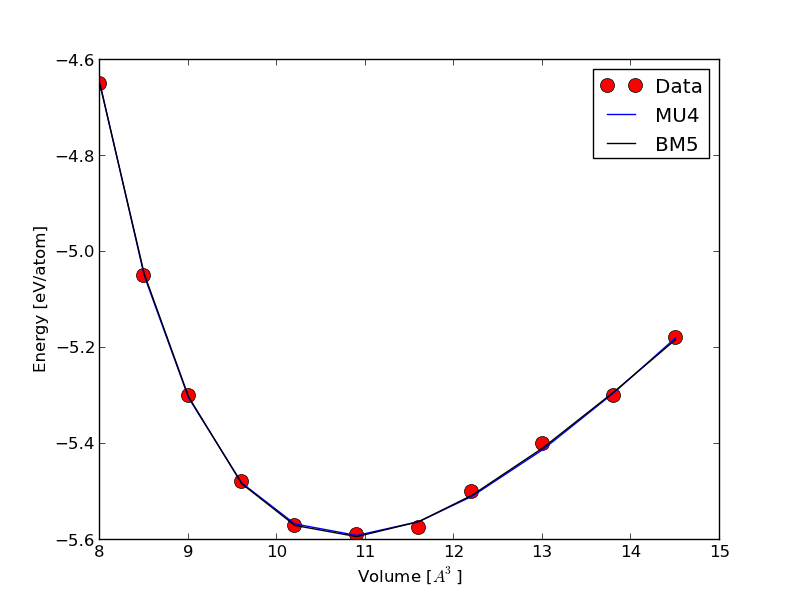
\includegraphics[scale=0.8]{eosfit_example.png}}
  	\caption{Fitting parameters of MU4 and BM5 models to experimental data.}
  	\label{fig:eosfit_example}
\end{figure}

To illustrate the relevance of computing confidence intervals, the models BM4 and VI4 were fit to the same data as above and the results are given in Table \ref{tbl:cicmp}. Note that the confidence intervals for VI4 are much \emph{tighter} than for BM4.
\begin{table}[H]
	\centering
	\caption{Optimal parameters and their confidence intervals for models BM4 and VI4 (95\% confidence).}
	\begin{tabular}{c | c c | c c}
		\hline
					&	\multicolumn{2}{c|}{BM4}						&	\multicolumn{2}{c}{VI4}					\\
		\hline
		Parameter	&	$p^*$		&	$ci$							&	$p^*$		&	$ci$						\\
		\hline
		$p_0$		&	$-6.0280$	&	$[-9.0572,\; -2.9987]$		&	$-5.5959$	&	$[-5.6031,\; -5.5888]$	\\
		$p_1$		&	$83.2840$	&	$[39.0626,\; 127.5053]$		&	$1.3132$		&	$[1.2808,\; 1.3456]$		\\
		$p_2$		&	$-782.4178$	&	$[-995.8613,\; -568.9743]$	&	$6.1059$		&	$[5.7164,\; 6.4953]$		\\
		$p_3$		&	$1885.1266$	&	$[1544.446,\; 2225.8071]$	&	$10.7855$	&	$[10.7400,\; 10.8310]$	\\
		\hline
	\end{tabular}
	\label{tbl:cicmp}
\end{table}
where $p = (a,\; b,\; c,\; d)$ for BM4 and $p = (E_0,\; B_0,\; B_0',\; V_0)$ for VI4.


%%%%%%%%%%%%%%%%%%%%%%%%%%%%%%%%%%%%%%%%%%%%%%%%%%%%%%%%%%%%%%%%%%%%%%%%%%%%%%%%%%%%%%%%%%%%%%%%%%%%%%%%%%%%%%%%%%%%%%%%%%%%%%%%%%%%%%%%%%%%

\bibliographystyle{plainnat}
\bibliography{MP1bib}

\end{document}
